%\documentclass{article}
%\usepackage[utf8]{inputenc}
%\usepackage{tikz,amsmath}
%\usetikzlibrary{positioning,shapes,topaths,calc}
%\begin{document}

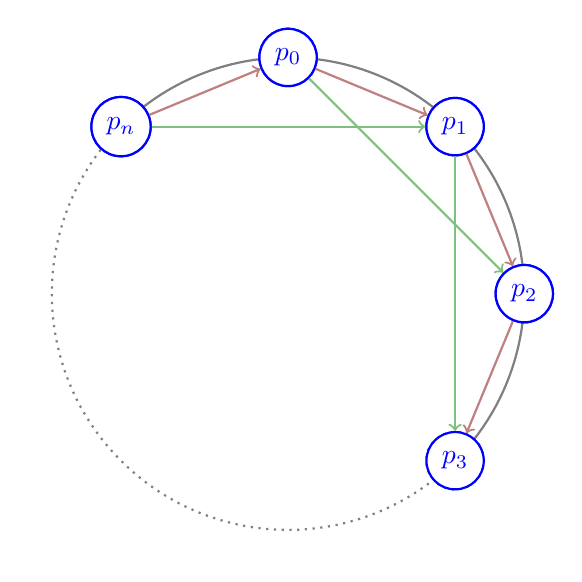
\begin{tikzpicture}
	[ thick,
	  core/.style={draw,circle,blue,fill=white}, 
	  ring/.style={gray},
	  dots/.style={ring,dotted},
	  inner/.style={->},
	  key/.style={font=\small} ]
	
	\draw[ring] node[core] (p0) {$p_0$} (0,0) arc (90:135:3cm) node[core] (pn) {$p_n$};
	\draw[dots] (pn) arc (135:315:3cm) node[core] (p3) {$p_3$};
	\draw[ring] (p3) arc (315:360:3cm) node[core] (p2) {$p_2$};
	\draw[ring] (p2) arc (0:45:3cm) node[core] (p1) {$p_1$};
	\draw[ring] (p1) arc (45:90:3cm) ;
	\node[core] at (p0) {$p_0$};
	\node[core] at (p1) {$p_1$};
	\node[core] at (p2) {$p_2$};
	\node[core] at (p3) {$p_3$};
	\node[core] at (pn) {$p_n$};
	
	\draw[inner,red!50!black!50] (pn) -- node[right,key] {} (p0);
	\draw[inner,red!50!black!50] (p0) -- node[right,key] {} (p1);
	\draw[inner,red!50!black!50] (p1) -- node[right,key] {} (p2);
	\draw[inner,red!50!black!50] (p2) -- node[right,key] {} (p3);
	
	\draw[inner,green!50!black!50] (pn) -- node[left,key] {} (p1);
	\draw[inner,green!50!black!50] (p0) -- node[left,key] {} (p2);
	\draw[inner,green!50!black!50] (p1) -- node[left,key] {} (p3);
	
\end{tikzpicture}

%\end{document}
